\documentclass{beamer}
\usetheme{Goettingen}
\usefonttheme[onlymath]{serif}

\usepackage[version=4]{mhchem}
\usepackage{graphicx}
\usepackage{empheq}
\usepackage[many]{tcolorbox}

\usepackage{tikz}
\usetikzlibrary{arrows,shapes,positioning,shadows,trees,matrix}
\tikzset{>=stealth}
\newcommand{\tikzmark}[3][]{\tikz[remember picture,baseline] \node [anchor=base,#1,](#2) {#3};}

\definecolor{red1}{RGB}{255,0,0}
\definecolor{red2}{RGB}{190,0,190}
\definecolor{red3}{RGB}{40,0,210}
\tcbset{highlight math style={enhanced, colframe=blue!20!black, colback=white, arc=4pt, boxrule=0.5pt}}

\title[Molecular Hydrophobicity Potential]
{%
    Implementing Molecular Hydrophobicity Potential Measurment for the Analysis of Dynamic Biomolecular Interactions
}
\date{\today}
\author[Pelg Bar Sapir]
{
    Peleg Bar Sapir\inst{1} \and \\
    Under supervision of Prof. Maria Andrea Mroginski\inst{2}
}
\institute[Freie Universit\"{a}t Berlin, Techniche Universit\"{a} Berlin]
{
    \inst{1}%
        Freie Universit\"{a}t Berlin
    \and
    \vskip-2mm
    \inst{2}%
        Techniche Universit\"{a}t Berlin
}

\begin{document}

\begin{frame}
    \titlepage
\end{frame}

\begin{frame}{Outline}
    \tableofcontents
\end{frame}

\section{Introduction}
\subsection{Hydrophobicity and log P}

\section{Molecular Hydrophobicity Potential}
\subsection{Potential}
\subsubsection{General form}

\begin{frame}{The MHP formula}
    \centering
    \begin{figure}
        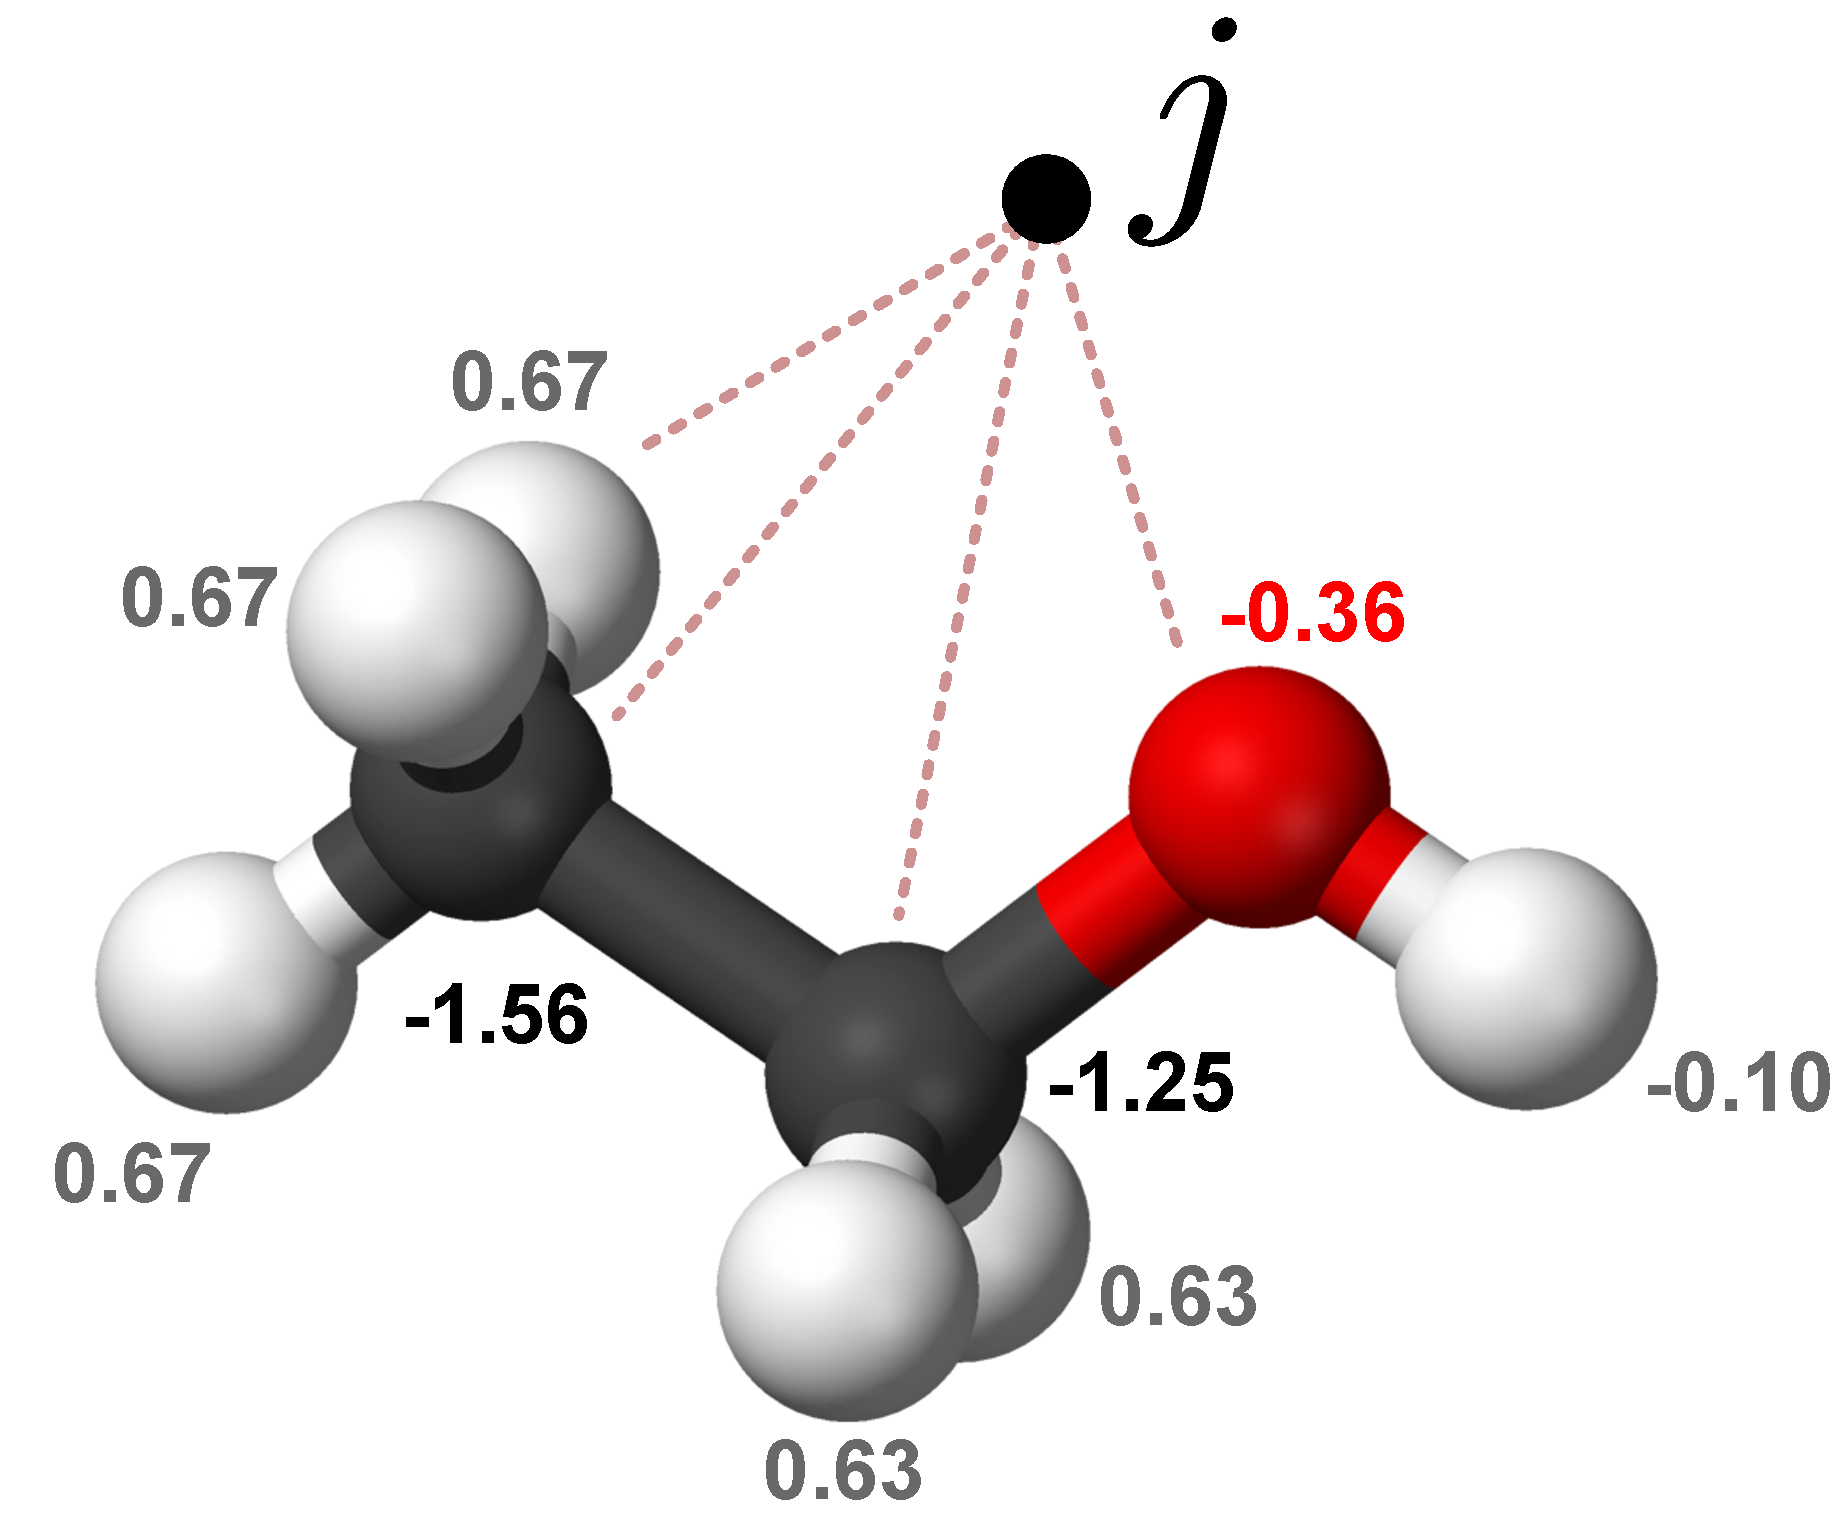
\includegraphics[width=0.4\textwidth]{mhp_visual1.eps}
    \end{figure}
    \begin{equation*}
        \text{MHP}\left(\mathbf{x'}\right)=
        \tikzmark[red1]{sum}{$\sum_{i=1}^{k}\limits$}
        \tikzmark[red2]{force}{$f_i$}\color{black}\cdot
        \tikzmark[red3]{distance}{$D\left(\left|\mathbf{x'}-\mathbf{x_i}\right|\right)$}
    \end{equation*}

    \begin{tikzpicture}[overlay, remember picture,node distance=1.5cm]
        \uncover<2-4>{\node[red1,xshift=1.0cm,yshift=0.5cm](sumdescr) [below left=of sum]{Summing over all atoms};}
        \uncover<2-4>{\draw[red1,->,thick] (sumdescr) to [in=-90,out=90] (sum);}
                        
        \uncover<3-4>{\node[red2] (forcedescr) [below = of force]{Force constants};}
        \uncover<3-4>{\draw[red2,->,thick] (forcedescr) to [in=-90,out=90] (force);}

        \uncover<4-4>{\node[red3,xshift=-2.0cm,yshift=0.5cm] (distancedescr) [below right = of distance]{Distance function};}
        \uncover<4-4>{\draw[red3,->,thick] (distancedescr) to [in=-90,out=90] (distance.south);}
    \end{tikzpicture}
\end{frame}

\subsubsection{Force constants}
\begin{frame}{Force constants}
    \centering
    \begin{tabular}{l l r}
        Type & Description & $f_i$ value \\
        \hline
            & \underline{C in:} &         \\
        3   & $\ce{CHR_3}$      & -0.6681 \\
        15  & $\ce{=CH_2}$      & -0.7866 \\
        36  & $\ce{R-CH-X}$     & -0.2405 \\
            & & \\
            & \underline{H attached to}:                            &         \\
        45  & $\ce{C_{sp^{3}}}$ having no X attached to next carbon &  0.7341 \\
        46  & $\ce{C_{sp^{3}}, C_{sp^{2}}}$                         &  0.6301 \\
        50  & Heteroatom                                            & -0.1036 \\
        52  & $\ce{C_{sp^{3}}}$ having 1 X attached to next carbon  &  0.6666 \\
            & & \\
            & \underline{O in}: &         \\
        56  & Alcohol           & -0.3567 \\
        58  & Ketone            & -0.0233 \\
        62  & \ce{O-}           & -0.7941 \\
        \hline
    \end{tabular}
\end{frame}

\subsubsection{Distance function}
\begin{frame}{Distance function}
    \centering
    \begin{minipage}[t]{0.48\linewidth}
        \centering
        Audry form
        \begin{empheq}[box=\tcbhighmath]{align*}
            D\left(x\right)=\frac{1}{1+x}
        \end{empheq}
    \end{minipage}
    \begin{minipage}[t]{0.48\linewidth}
        \centering
        Exponential decay form
        \begin{empheq}[box=\tcbhighmath]{align*}
            D\left(x\right)=e^{-\alpha x}
        \end{empheq}
    \end{minipage}
    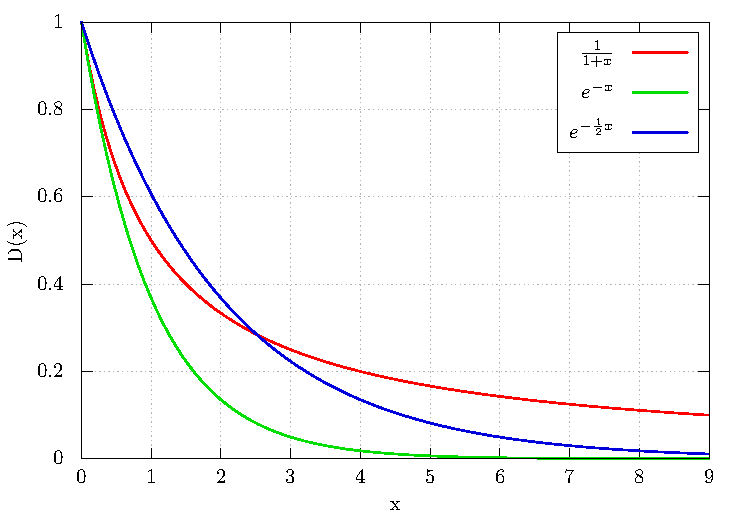
\includegraphics[scale=0.65]{dist_funcs.pdf}    
\end{frame}

\subsection{Surface}
\subsubsection{Solvent accesible surface}
\begin{frame}{Solvent accesible surface}
\end{frame}

\subsubsection{Evenly distributed points}
\begin{frame}{Evenly distributed points}
\end{frame}

\subsubsection{Integration}
\begin{frame}{Integration}
\end{frame}

\end{document}
